\section{Frozen stars: a sharp percolation threshold}
\label{sec:static}

\paragraph{Exact reduction.} With stars fixed, the smallest range that reaches
star $j$ from the Sun is the \emph{bottleneck} of the best path: the minimum
over paths of the largest hop. On a complete Euclidean graph this minimax path
runs along the minimum spanning tree (MST). One MST, built from a $k$-NN graph
and verified against the dense MST, gives the bottleneck of all \NStars\ stars
at once. The reachable fraction at range $r$ is the fraction of stars whose
bottleneck is $\le r$.

\begin{figure}[t]
\centering
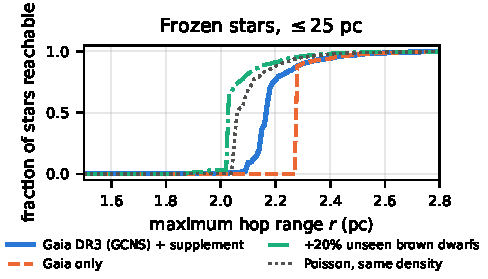
\includegraphics[width=\linewidth]{figures/percolation.pdf}
\caption{Fraction of the \NEval\ stars within \EvalRadius~pc reachable from the
Sun with frozen stars, against the maximum single hop $r$. The transition is
abrupt. With Gaia alone (dashed) the Sun's \PocketGaiaSize-star pocket holds
everything until $r$ reaches \PocketBridge~pc. Unseen brown dwarfs (dash-dot,
+20\%) and a Poisson field of equal density (dotted) shift the threshold
slightly lower.}
\label{fig:percolation}
\end{figure}

\paragraph{The threshold.} Reach jumps from almost nothing to almost everything
over a narrow band of $r$ (Figure~\ref{fig:percolation}). Ten percent of the
stars within \EvalRadius~pc are reachable at $r_{10}=\RTen$~pc, half at
$r_{50}=\RFifty$~pc (bootstrap 95\% CI over Gaia astrometric errors:
\RFiftyLo--\RFiftyHi~pc), and 90\% at $r_{90}=\RNinety$~pc. The median
nearest-neighbour distance is \NNMedian~pc, so a ship must out-range the
typical spacing by a factor of about two. The threshold barely depends on
the evaluation radius: $r_{50}$ lies between \RFiftySweepMin\ and
\RFiftySweepMax~pc for radii of 10--25~pc. This is percolation. A Poisson field
of the same density gives $r_{50}=\RFiftyPoisson$~pc, close to the
infinite-volume continuum value of \RcPoisson~pc \cite{lorenz2001precise}. The
real neighbourhood is \PctAbovePoisson\% harder to cross than random, a mild
cost of its clustering.

\paragraph{The Sun's pocket.} With Gaia alone, the bottleneck for almost every
star is the same hop. The Sun, Proxima, Barnard's star and Ross~154 form an
island whose shortest way out is a \PocketBridge~pc jump from Ross~154. Adding
Luhman~16 and WISE~0855, the two nearest brown dwarfs, both invisible to Gaia,
opens the pocket, and the threshold becomes a property of the whole field. The
lesson is that the \emph{least visible} objects can be the most important
stepping stones. Injecting a random population of unseen brown dwarfs at 20\%
(30\%) of the stellar number, roughly the ratio in the 20-pc census
\cite{kirkpatrick2021field}, lowers $r_{50}$ to \RFiftyBDTwenty\
(\RFiftyBDThirty)~pc, a \PctBDTwenty\% reduction at 20\%.

\paragraph{Route shape.} Just above threshold, at $r_{90}$, the shortest routes
are long detours. The median route flies \StretchMedian$\times$ the
straight-line distance in \HopsMedian\ hops. Section~\ref{sec:engineering}
shows that this regime defeats simple greedy pilots.

\begin{figure}[t]
\centering
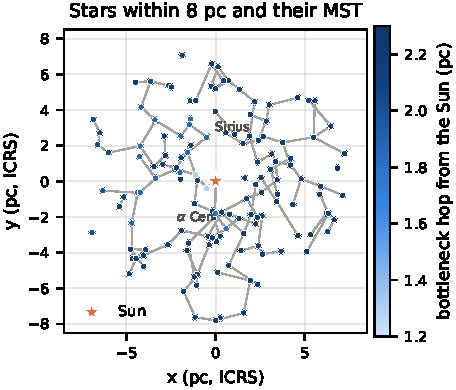
\includegraphics[width=0.92\linewidth]{figures/map.pdf}
\caption{The 3D minimum spanning tree of stars within 8~pc, projected on the
ICRS $x$--$y$ plane, coloured by each star's bottleneck hop from the Sun.
Nearly every star shares the same bottleneck.}
\label{fig:map}
\end{figure}
